\let\negmedspace\undefined
\let\negthickspace\undefined
\documentclass[journal]{IEEEtran}
\usepackage[a5paper, margin=10mm, onecolumn]{geometry}
%\usepackage{lmodern} % Ensure lmodern is loaded for pdflatex
\usepackage{tfrupee} % Include tfrupee package

\setlength{\headheight}{1cm} % Set the height of the header box
\setlength{\headsep}{0mm}  % Set the distance between the header box and the top of the text

\usepackage{gvv-book}
\usepackage{gvv}
\usepackage{cite}
\usepackage{amsmath,amssymb,amsfonts,amsthm}
\usepackage{algorithmic}
\usepackage{graphicx}
\usepackage{textcomp}
\usepackage{xcolor}
\usepackage{txfonts}
\usepackage{listings}
\usepackage{enumitem}
\usepackage{mathtools}
\usepackage{gensymb}
\usepackage{comment}
\usepackage[breaklinks=true]{hyperref}
\usepackage{tkz-euclide} 
\usepackage{listings}
% \usepackage{gvv}                                        
\def\inputGnumericTable{}                                 
\usepackage[latin1]{inputenc}                                
\usepackage{color}                                            
\usepackage{array}                                            
\usepackage{longtable}                                       
\usepackage{calc}
\usepackage{caption}
\usepackage{multirow}                                         
\usepackage{hhline}                                           
\usepackage{ifthen}                                           
\usepackage{lscape}
\usepackage{tikz}
\usetikzlibrary{patterns}

\title{\textbf{GATE 2025 ES}}
\author{ee25btech11035 - Kushal B N}
\date{}

\begin{document}
\maketitle

\section*{General Aptitude (GA)}

\subsection*{Q.1 -- Q.5 Carry ONE mark Each}

\begin{enumerate}
\item If `$\rightarrow$' denotes increasing order of intensity, then the meaning of the words
\begin{align}
[\text{sick} \rightarrow \text{infirm} \rightarrow \text{moribund}]
\end{align}
is analogous to 
\begin{align}
[\text{silly} \rightarrow \_\_\_\_\_\_ \rightarrow \text{daft}]
\end{align}
Which one of the given options is appropriate to fill the blank?
\hfill\brak{GATE~ES~2025}

\begin{multicols}{2}
\begin{enumerate}
\item frown
\item fawn
\item vein
\item vain
\end{enumerate}
\end{multicols}

\item The 15 parts of the given figure are to be painted such that no two adjacent parts with shared boundaries (excluding corners) have the same color. The minimum number of colors required is
\hfill\brak{GATE~ES~2025}

\begin{figure}[H]
    \centering
    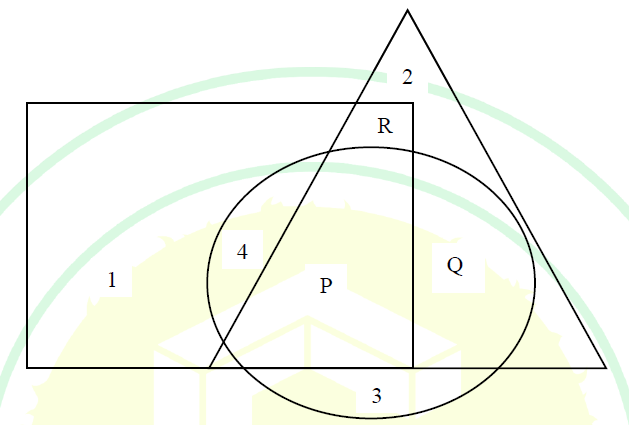
\includegraphics[width=0.5\columnwidth]{figs/fig1.png}
    \label{fig:placeholder}
\end{figure}

\begin{multicols}{4}
\begin{enumerate}
\item 4
\item 3
\item 5
\item 6
\end{enumerate}
\end{multicols}

\item How many 4-digit positive integers divisible by 3 can be formed using only the digits
$\cbrak{1, 3, 4, 6, 7}$, such that no digit appears more than once in a number?
\hfill\brak{GATE~ES~2025}

\begin{multicols}{4}
\begin{enumerate}
\item 24
\item 48
\item 72
\item 12
\end{enumerate}
\end{multicols}

\item The sum of the following infinite series is

\begin{align*}
2 + \frac{1}{2} + \frac{1}{3} + \frac{1}{4} + \frac{1}{8} + \frac{1}{9} + \frac{1}{16} + \frac{1}{27} + \cdots
\end{align*}
\hfill\brak{GATE~ES~2025}

\begin{multicols}{4}
\begin{enumerate}
\item $\frac{11}{3}$
\item $\frac{7}{2}$
\item $\frac{13}{4}$
\item $\frac{9}{2}$
\end{enumerate}
\end{multicols}

\item In an election, the share of valid votes received by the four candidates A, B, C, and D is represented by the pie chart shown. The total number of votes cast in the election were 1,15,000, out of which 5,000 were invalid. 
\hfill\brak{GATE~ES~2025}

\begin{figure}[H]
    \centering
    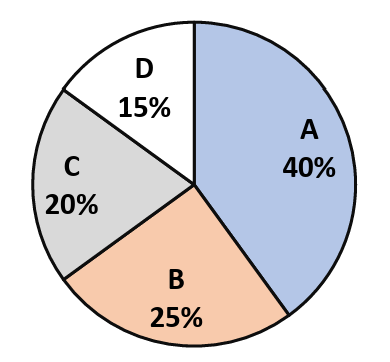
\includegraphics[width=0.5\columnwidth]{figs/fig2.png}
    \caption*{\textbf{Share of valid votes}}
    \label{fig:placeholder}
\end{figure}

Based on the data provided, the total number of valid votes received by the candidates B and C is
\hfill\brak{GATE~ES~2025}

\begin{multicols}{2}
\begin{enumerate}
\item 45,000
\item 49,500
\item 51,750
\item 54,000
\end{enumerate}
\end{multicols}

\subsection*{Q.6 -- Q.10 Carry TWO marks Each}

\item Thousands of years ago, some people began dairy farming. This coincided with a number of mutations in a particular gene that resulted in these people developing the ability to digest dairy milk.

Based on the given passage, which of the following can be inferred?
\hfill\brak{GATE~ES~2025}

\begin{enumerate}
\item All human beings can digest dairy milk.
\item No human being can digest dairy milk.
\item Digestion of dairy milk is essential for human beings.
\item In human beings, digestion of dairy milk resulted from a mutated gene.
\end{enumerate}

\item The probability of a boy or a girl being born is $\frac{1}{2}$. For a family having only three children, what is the probability of having two girls and one boy?
\hfill\brak{GATE~ES~2025}

\begin{multicols}{4}
\begin{enumerate}
\item $\frac{3}{8}$
\item $\frac{1}{8}$
\item $\frac{1}{4}$
\item $\frac{1}{2}$
\end{enumerate}
\end{multicols}

\item Person 1 and Person 2 invest in three mutual funds A, B, and C. The amounts they invest in each of these mutual funds are given in the table.

\begin{center}
\begin{tabular}{|c|c|c|c|}
 \hline & Mutual fund A & Mutual fund B & Mutual fund C \\
 \hline Person 1 & \rupee 10,000 & \rupee 20,000 & \rupee 20,000 \\
 \hline Person 2 & \rupee 20,000 & \rupee 15,000 & \rupee 15,000 \\
 \hline
\end{tabular}
\end{center}

At the end of one year, the total amount that Person 1 gets is \rupee 500 more than Person 2. The annual rate of return for the mutual funds B and C is 15\% each. What is the annual rate of return for the mutual fund A?
\hfill\brak{GATE~ES~2025}

\begin{multicols}{2}
\begin{enumerate}
\item 7.5\%
\item 10\%
\item 15\%
\item 20\%
\end{enumerate}
\end{multicols}

\item Three different views of a dice are shown in the figure below.
\begin{figure}[H]
    \centering
    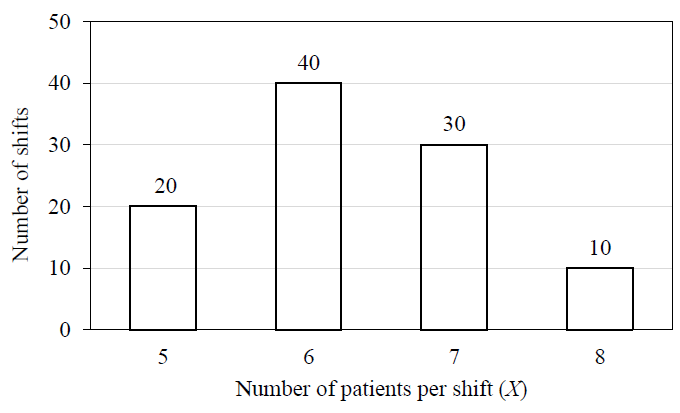
\includegraphics[width=0.5\columnwidth]{figs/fig3.png}
    \caption{Different Views of a dice}
    \label{fig:placeholder}
\end{figure}

The piece of paper that can be folded to make this dice is

\hfill\brak{GATE~ES~2025}
\begin{enumerate}

\item 
\begin{figure}[H]
    \centering
    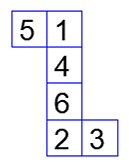
\includegraphics[width=0.25\textwidth]{figs/fig4.png}
\end{figure}

\item 
\begin{figure}[H]
    \centering
    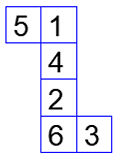
\includegraphics[width=0.25\columnwidth]{figs/fig5.png}
\end{figure}

\item 
\begin{figure}[H]
    \centering
    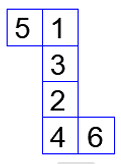
\includegraphics[width=0.25\columnwidth]{figs/fig6.png}
\end{figure}

\item 
\begin{figure}[H]
    \centering
    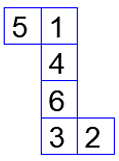
\includegraphics[width=0.25\columnwidth]{figs/fig7.png}
\end{figure}

\end{enumerate}

\item Visualize two identical right circular cones such that one is inverted over the other and they share a common circular base. If a cutting plane passes through the vertices of the assembled cones, what shape does the outer boundary of the resulting cross-section make?
\hfill\brak{GATE~ES~2025}

\begin{multicols}{2}
\begin{enumerate}
\item A rhombus
\item A triangle
\item An ellipse
\item A hexagon
\end{enumerate}
\end{multicols}

\section*{Environmental Science and Engineering (ES)}

\subsection*{Q.11 -- Q.35 Carry ONE mark Each}

\item Ten cards in a pack are numbered as 1, 2, 3, \dots, 10. The probability of drawing a card with an even number or a number which is a multiple of 5 from the pack is \_\_\_\_\_\_.
\hfill\brak{GATE~ES~2025}

\begin{multicols}{2}
\begin{enumerate}
\item $\frac{4}{10}$
\item $\frac{6}{10}$
\item $\frac{2}{10}$
\item $\frac{3}{10}$
\end{enumerate}
\end{multicols}

\item Hardness in water is NOT caused by \_\_\_\_\_\_.
\hfill\brak{GATE~ES~2025}

\begin{multicols}{2}
\begin{enumerate}
\item $Ca^{2+}$
\item $Si^{2+}$
\item $Mg^{2+}$
\item $CO_3^{2-}$
\end{enumerate}
\end{multicols}

\item The maximum coordination number of $Sn^{4+}$ is \_\_\_\_\_\_.
\hfill\brak{GATE~ES~2025}

\begin{multicols}{2}
\begin{enumerate}
\item 4
\item 8
\item 6
\item 2
\end{enumerate}
\end{multicols}

\item Rod shaped bacterial cells are called \_\_\_\_\_\_.
\hfill\brak{GATE~ES~2025}

\begin{multicols}{2}
\begin{enumerate}
\item Bacilli
\item Cocci
\item Spirilla
\item Diplococci
\end{enumerate}
\end{multicols}

\item Tuberculosis is predominantly caused by \_\_\_\_\_\_\_.
\hfill\brak{GATE~ES~2025}

\begin{multicols}{2}
\begin{enumerate}
\item Entamoeba histolytica
\item Salmonella typhi
\item Mycobacterium bovis
\item Bacillus cereus
\end{enumerate}
\end{multicols}

\item Which one of the following conversions belongs to nonsymbiotic nitrogen fixation?
\hfill\brak{GATE~ES~2025}

\begin{enumerate}
\item Atmospheric nitrogen to ammonia by \textit{Rhizobium} bacteria in nodules attached to roots of legumes
\item Atmospheric nitrogen to ammonia by \textit{Azotobacter} species
\item Nitrate to gaseous nitrogen under anaerobic conditions
\item Nitrate to ammonia under aerobic conditions
\end{enumerate}

\item Crown corrosion of reinforced cement concrete sewer is caused by \_\_\_\_\_\_.
\hfill\brak{GATE~ES~2025}

\begin{multicols}{2}
\begin{enumerate}
\item sulfur oxidizing bacteria
\item iron oxidizing bacteria
\item denitrifying bacteria
\item fermentative bacteria
\end{enumerate}
\end{multicols}

\item The processes of removal of particles in a rapid sand filter with their description is given in the table.

\begin{center}

\renewcommand{\arraystretch}{1.2}

\begin{tabular}{|c|p{9cm}|}
\hline
\textbf{Process} & \textbf{Description} \\
\hline
(i) Straining & P: Removes only particles in the water large enough to get \\ & caught in the pores of the filter \\
\hline
(ii) Sedimentation & Q: Larger and heavier particles do not follow the fluid \\& streamline around the sand grain and settle on the grain \\
\hline
(iii) Interception & R: Particles that do follow the streamline, but are too large \\& and are caught because they brush up against the sand grains \\
\hline
(iv) Diffusion & S: Very small particles are experiencing Brownian motion \\& and may collide with the sand grains by chance \\
\hline
\end{tabular}
\end{center}

Select the correct match.
\hfill\brak{GATE~ES~2025}

\begin{multicols}{2}
\begin{enumerate}
\item i-S; ii-P; iii-Q; iv-R
\item i-Q; ii-R; iii-S; iv-P
\item i-R; ii-S; iii-P; iv-Q
\item i-P; ii-Q; iii-R; iv-S
\end{enumerate}
\end{multicols}

\item The environmental temperature increases by $6\celsius/km$ with height at a particular location. The stability condition of the atmosphere at the location is \_\_\_\_\_.
\hfill\brak{GATE~ES~2025}

\begin{multicols}{2}
\begin{enumerate}
\item stable
\item unstable
\item inversion
\item neutral
\end{enumerate}
\end{multicols}

\item As per the United Nations agenda for sustainable development adopted in September 2015, the number of Sustainable Development Goals (SDGs) are \_\_\_\_\_\_ and the proposed target year to achieve them is \_\_\_\_\_\_.
\hfill\brak{GATE~ES~2025}

\begin{multicols}{2}
\begin{enumerate}
\item 15; 2035
\item 17; 2030
\item 20; 2050
\item 18; 2047
\end{enumerate}
\end{multicols}

\item Which one of the following is \textbf{NOT} a greenhouse gas?
\hfill\brak{GATE~ES~2025}

\begin{multicols}{2}
\begin{enumerate}
\item $CO_2$
\item $CH_4$
\item $H_2S$
\item $H_2O$
\end{enumerate}
\end{multicols}

\item As per the United Nations Environmental Program (UNEP) guidelines 2004, the maximum size of microplastics is \_\_\_\_\_\_.
\hfill\brak{GATE~ES~2025}

\begin{multicols}{2}
\begin{enumerate}
\item $10 mm$
\item $5 mm$
\item $10\mu m$
\item $5 \mu m$
\end{enumerate}
\end{multicols}

\item The costliest functional element in an urban centralized Municipal Solid Waste management infrastructure for a typical Indian Tier I city is \_\_\_\_\_\_\_.
\hfill\brak{GATE~ES~2025}

\begin{multicols}{2}
\begin{enumerate}
\item biological treatment
\item collection and transport
\item disposal in a sanitary landfill
\item thermal treatment
\end{enumerate}
\end{multicols}

\item The eigen values of the matrix $ \myvec{4 & 3 \\ 3 & 4}$ are \hfill\brak{GATE~ES~2025}

\begin{multicols}{4}
\begin{enumerate}
\item 1
\item 2
\item 7
\item 4
\end{enumerate}
\end{multicols}

\item If $X$ is a vector, and $A$ and $B$ are linear operators; then the correct mathematical relationship(s) is/are \hfill\brak{GATE~ES~2025}

\begin{multicols}{2}
\begin{enumerate}
\item $\brak{A+B}X = AX + BX$
\item $\brak{\lambda A}X = \lambda\brak{AX}$
\item $\brak{AB}X = A\brak{BX}$
\item $\brak{A+B}X = A^TX + B^TX$
\end{enumerate}
\end{multicols}

\item In the context of fluid flow, which of the following statement(s) is/are correct? \hfill\brak{GATE~ES~2025}

\begin{enumerate}
\item \textit{Streamline} is a line, tangent to which at any point gives the direction of the velocity vector
\item \textit{Streakline} is the actual path traversed by a given fluid particle in an unsteady flow
\item \textit{Streakline} and \textit{streamline} are same for a steady flow
\item \textit{Pathline} and \textit{streamline} are same for a steady flow
\end{enumerate}

\item In a rectangular open channel, the flow is critical, and the flow depth is $2m$. Select the correct statement(s) \hfill\brak{GATE~ES~2025}

\begin{enumerate}
\item Specific energy for the flow is $3.0m$
\item Specific energy for the flow is $2.0m$
\item Froude number is $1.0$
\item Froude number is $1.5$
\end{enumerate}

\item With respect to particle settling in wastewater treatment systems; the correct statement(s) is/are \hfill\brak{GATE~ES~2025}

\begin{enumerate}
\item Settling in grit chamber and primary sedimentation tanks are examples of Type-I settling
\item Settling in primary sedimentation tank and secondary sedimentation tank are examples of Type-II settling
\item Settling in grit chamber is an example of Type-I settling, whereas settling in primary sedimentation tank is an example of Type-II settling
\item Settling in secondary sedimentation tank is an example of Type-III settling, whereas settling in primary sedimentation tank is an example of Type-II settling
\end{enumerate}

\item The equipment that can be used to control particulate air pollution in an industrial unit is/are \hfill\brak{GATE~ES~2025}

\begin{multicols}{2}
\begin{enumerate}
\item Electrostatic precipitator
\item Cyclone separator
\item Gravity settler
\item Incinerator
\end{enumerate}
\end{multicols}

\item Which is/are the secondary air pollutant(s)? \hfill\brak{GATE~ES~2025}

\begin{multicols}{2}
\begin{enumerate}
\item $O_3$
\item $HNO_3$
\item $CO_2$
\item $H_2SO_4$
\end{enumerate}
\end{multicols}

\item As per the Hazardous Waste (Management and Handling) Rules, 2016, of India, which is/are the characteristic(s) that must be exhibited by a waste to be classified as a ``characteristic'' hazardous waste? \hfill\brak{GATE~ES~2025}

\begin{multicols}{2}
\begin{enumerate}
\item Ignitability
\item Reactivity
\item Radioactivity
\item Toxicity
\end{enumerate}
\end{multicols}

\item $f\brak{x} = x^3 - 4.5x^2 - 12x$ has a local maximum at $x =$ \_\_\_\_\_\_ \textit{(an integer value)} in the range $x = -2$ to $+2$. \hfill\brak{GATE~ES~2025}

\item Consider the equation
\begin{align*}
\frac{dy}{dx} - x^2 + e^x = 0
\end{align*}
with $y = 1$ at $x = 0$. The value of $y$ at $x = 1$ is \_\_\_\_\_\_ \textit{(rounded off to 2 decimal places)}. Take the value of $e$ (base of natural logarithm) as 2.7. \hfill\brak{GATE~ES~2025}

\item A municipal solid waste digester generates $1000\,\text{kg}$ of methane gas. The volume of the tank needed to store this gas at $30\celsius$ and $3$ atmospheric pressure is \_\_\_\_\_\_ liters \textit{(an integer value)}. Use $R = 0.082$ L-atm/mole-K, Atomic weights of $C=12$, and $H=1$. \hfill\brak{GATE~ES~2025}

\item A Class-A pan was setup adjacent to a lake for measuring evaporation losses in the lake. The depth of water in the pan at the beginning of a certain week was $250mm$. In that week, there was a rainfall event with $10mm$ depth. Water depth in the pan at the end of the week was $240mm$. The pan coefficient is $0.8$. The estimated lake evaporation during the week was \underline{\phantom{answer}} mm \textit{(an integer value)}. \hfill\brak{GATE~ES~2025}

\subsection*{Q.36 -- Q.65 Carry TWO marks Each}

\item A population (with mean $\mu$) follows normal distribution. Ten samples ($N$) are drawn at random with a mean value of ``x'' and standard deviation of ``S''. Following table provides the confidence limits, $C(t)$ of the cumulative probability function for Student's t - distribution two-tailed test with degree of freedom, $D$. Which one of the following expression is correct for testing the null hypothesis $H_o$: $\mu$ = 0 at 10\% significance level?
\hfill\brak{GATE~ES~2025}
\begin{table}[H]
\centering
\begin{tabular}{|c|c|c|c|}
\hline
\textbf{D} & \multicolumn{3}{c|}{\textbf{C(t)}} \\
\cline{2-4}
& \textbf{0.9} & \textbf{0.95} & \textbf{0.975} \\
\hline
9 & 1.38 & 1.83 & 2.26 \\
\hline
10 & 1.37 & 1.81 & 2.23 \\
\hline
11 & 1.36 & 1.80 & 2.20 \\
\hline
\end{tabular}
\end{table}
\begin{enumerate}
\item $-1.81 < \frac{x}{\frac{S}{\sqrt{N-1}}} < 1.81$
\item $-1.83 < \frac{x}{\frac{S}{\sqrt{N-1}}} < 1.83$
\item $-1.37 < \frac{x}{\frac{S}{\sqrt{N-1}}} < 1.37$
\item $-2.23 < \frac{x}{\frac{S}{\sqrt{N-1}}} < 2.23$
\end{enumerate}

\item Which one is the solution $y(x)$ for the following ordinary differential equation and the specified boundary conditions? \\
\begin{align*}
\frac{d^2y}{dx^2} - 3\frac{dy}{dx} + 2y = 2e^{-x}; y(0) = 2; \brak{\frac{dy}{dx}}_{x=0} = 1
\end{align*}

\hfill\brak{GATE~ES~2025}
\begin{enumerate}
\item $y(x) = \frac{1}{3}e^{-x} - 2e^{x} - \frac{1}{3}e^{2x}$
\item $y(x) = \frac{1}{3}e^{x} + 2e^{x} - \frac{1}{3}e^{2x}$
\item $y(x) = \frac{1}{3}e^{-x} + 2e^{-x} - \frac{1}{3}e^{2x}$
\item $y(x) = \frac{1}{3}e^{-x} + 2e^{x} - \frac{1}{3}e^{2x}$
\end{enumerate}

\item A saturated $CaCO_{3}$ stock solution is existing at 25$^{\circ}$C. In one experiment (i) 25 g $Na_{2}CO_{3}$ is added to the stock solution. In another experiment (ii) 25 g $Na_{2}SO_{4}$ is added to the stock solution. Select the correct statement from the following.
\hfill\brak{GATE~ES~2025}
\begin{enumerate}
\item Addition of (i) increases the concentration of $Ca^{2+}$ and addition of (ii) decreases the concentration of $Ca^{2+}$
\item Addition of (i) decreases the concentration of $Ca^{2+}$ and addition of (ii) increases the concentration of $Ca^{2+}$
\item Addition of (i) and (ii) increase the concentration of $Ca^{2+}$
\item Addition of (i) and (ii) decrease the concentration of $Ca^{2+}$
\end{enumerate}

\item Consider second order kinetics ($r_{c} = -kC^2$) under steady state condition. The ratio of volume of a complete mixed reactor (CMR) to that of a plug flow reactor (PFR) to achieve 90\% reduction in the concentration is \_\_\_\_\_\_\_. Inlet concentrations in both the reactors are same.
\hfill\brak{GATE~ES~2025}
\begin{enumerate}
\item 10.0
\item 1.0
\item 0.1
\item 2.3
\end{enumerate}

\item Consider two horizontal layers of an aquifer as shown in \figref{fig8}. Each layer is isotropic and homogeneous. Flow is parallel to the stratification. Thickness and horizontal hydraulic conductivity of layer-1 are $h_{1}$ and $K_{1}$, respectively. Thickness and horizontal hydraulic conductivity of layer-2 are $h_{2}$ and $K_{2}$, respectively, where $h_{1}$ is not equal to $h_{2}$. The equivalent horizontal conductivity $K_{x}$ for the aquifer system is given by \_\_\_\_\_\_\_.
\hfill\brak{GATE~ES~2025}
\begin{figure}[H]
    \centering
    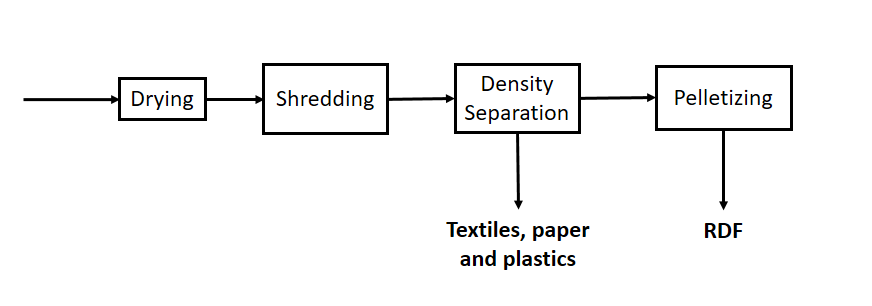
\includegraphics[width=0.5\linewidth]{figs/fig8.png}
    \caption{}
    \label{fig8}
\end{figure}
\begin{enumerate}
\item $K_{x} = \frac{K_{1} h_{1} + K_{2} h_{2}}{h_{1} + h_{2}}$
\item $K_{x} = \frac{K_{1} + K_{2}}{2}$
\item $K_{x} = \frac{K_{1} h_{2} + K_{2} h_{1}}{h_{1} + h_{2}}$
\item $K_{x} = \sqrt{K_{1}K_{2}}$
\end{enumerate}

\item A gravity settling chamber of height `H' and length `L' is designed to control particulate air pollution. In the chamber, the horizontal velocity of air flow is `$V_{h}$' and terminal settling velocity of the target particle is `$V_{t}$'. Which one of the following expressions is the correct concept used to calculate the minimum size of the target particle that will be removed with 100\% efficiency?
\hfill\brak{GATE~ES~2025}
\begin{enumerate}
\item $\frac{V_{t}}{L} = \frac{V_{h}}{H}$
\item $V_{h} \times V_{t} = L \times H$
\item $V_{h} = V_{t} \times L \times H$
\item $\frac{V_{t}}{H} = \frac{V_{h}}{L}$
\end{enumerate}

\item Consider the function $f(x) = \ln(\sin(x))$. Expand $f(x+h)$ using Taylor's series. In this context, the correct statement(s) is/are
\hfill\brak{GATE~ES~2025}
\begin{enumerate}
\item Second term in the Taylor's series i.e., the term which includes h is: $h \cdot \ln(\sin(x))$
\item First term is $\ln(\sin(x))$
\item Third term in the Taylor's series i.e., the term which includes $h^2$ is: $-\frac{h^2}{2(\sin(x))^2}$
\item Third term in the Taylor's series i.e., the term which includes $h^2$ is: $\frac{2h^2}{(\sin(x))^2}$
\end{enumerate}

\item Enzymes with the class of enzymes are listed in the table.
\hfill\brak{GATE~ES~2025}
\begin{table}[H]
\centering
\begin{tabular}{|l|l|}
\hline
\textbf{Enzyme} & \textbf{Class of Enzyme} \\
\hline
(a) Lactate dehydrogenase & (i) Isomerases \\
\hline
(b) Alanine racemase & (ii) Transferases \\
\hline
(c) Lipase & (iii) Oxidoreductases \\
\hline
(d) Hexokinase & (iv) Hydrolases \\
\hline
\end{tabular}
\end{table}
Select the correct match(es)
\begin{enumerate}
\item (a) - (iii); (b) - (i)
\item (c) - (iv); (d) - (ii)
\item (a) - (ii); (b) - (iv)
\item (c) - (iii); (d) - (i)
\end{enumerate}

\item With reference to disinfection, which of the following statement(s) is/are {CORRECT}?
\hfill\brak{GATE~ES~2025}
\begin{enumerate}
\item Ethanol damages lipid structures in the bacterial cell membrane.
\item Mercuric chloride inactivates cellular enzymes containing sulfhydryl groups.
\item Glutaraldehyde inactivates protein.
\item Isopropyl alcohol cannot be used as a disinfectant.
\end{enumerate}

\item Which of the following statement(s) is/are CORRECT?
\hfill\brak{GATE~ES~2025}
\begin{enumerate}
\item DNA is composed of nucleotides.
\item Five types of nitrogenous bases occur in DNA.
\item Each phosphate is attached to two deoxyribose units in a single strand of DNA.
\item The ratio of adenine to guanine is always 1:1 in a double stranded DNA.
\end{enumerate}

\item The Streeter-Phelp's oxygen sag equation for a river is based on a few assumptions. The correct assumption(s) is/are
\hfill\brak{GATE~ES~2025}
\begin{enumerate}
\item At any instant the deoxygenation rate is directly proportional to the amount of oxidizable organic material present.
\item At any instant the deoxygenation rate is inversely proportional to the amount of oxidizable organic material present.
\item The reoxygenation rate is directly proportional to the dissolved oxygen deficit.
\item The reoxygenation rate and deoxygenation rate are directly proportional to the saturation concentration of dissolved oxygen.
\end{enumerate}

\item Water is flowing \textbf{FULL} through a rectangular tunnel of size 3 m (width) $\times$ 2 m (height). The average velocity of flow is $1 m/s.$ The frictional head loss is observed to be 1 m per km. Consider acceleration due to gravity ($g$) as $10 m/s^2$. The correct statement(s) is/are
\hfill\brak{GATE~ES~2025}
\begin{enumerate}
\item Hydraulic radius is 0.6 m
\item Darcy-Weisbach friction factor is 0.048
\item Hydraulic radius is 2 m
\item Darcy-Weisbach friction factor is 0.024
\end{enumerate}

\item Based on the ISO 14040 methodology for Life Cycle Assessment, match the terms with the descriptions in the table.
\hfill\brak{GATE~ES~2025}
\begin{table}[H]
\centering
\begin{tabular}{|l|l|}
\hline
\textbf{Term} & \textbf{Description} \\
\hline
(a) Goal and Scope & (i) Based on the product or system, the \\& comparative unit must be carefully defined and \\& be same for all scenarios \\
\hline
(b) Functional Unit & (ii) The problem is described, and the objective of \\& the study are defined \\
\hline
(c) Life Cycle Inventory & (iii) Evaluates the environmental implications due \\& to the inventorized emissions \\
\hline
(d) Impact Assessment & (iv) Process based approach and input-output approach \\
\hline
\end{tabular}
\end{table}
The correct match(es) is/are
\begin{enumerate}
\item (a)-(ii); b-(i);
\item (a)-(iii), b-(i)
\item (c)-(iii), (d)-(iv)
\item (c)-(iv), (d)-(iii)
\end{enumerate}

\item Consider the equation for a curve, $y = f(x) = x^2 + x$. The area enclosed by the curve, the $x$-axis ($y = 0$ line); the vertical lines passing through $x = 1$ and $x = 2$ is \_\_\_\_\_\_\_ \textit{(rounded off to 2 decimal places)}.
\hfill\brak{GATE~ES~2025}

\item The pH of a solution containing 0.1M of acetic acid and 0.05 M of sodium acetate is \_\_\_\_\_\_\_ \textit{(rounded off to 2 decimal places)}. The $pK_{a}$ value of ionization of acetic acid is 4.76.
\hfill\brak{GATE~ES~2025}

\item The ionic strength of a solution containing 0.01M of $CaCl_{2}$ and 0.001M of $Na_{2}SO_{4}$ is \_\_\_\_\_\_\_ M \textit{(rounded off to 3 decimal places)}.
\hfill\brak{GATE~ES~2025}

\item The concentration of Ozone corresponding to a mixing ratio of 120 ppbv at pressure of 1 atmosphere and temperature of 25$^{\circ}$C is \_\_\_\_\_\_\_ $\mu g/m^3$ \textit{(rounded off to 1 decimal place)}. Atomic weight of oxygen = 16; $R$= 8.314 J/K-g.mole.
\hfill\brak{GATE~ES~2025}

\item One million liters per day (MLD) of wastewater with a soluble BOD of 200 mg/L is treated in an activated sludge process. The BOD of treated wastewater is 20 mg/L. The observed yield coefficient of the biological system is 0.35. The daily biomass generation in the system is \_\_\_\_\_\_\_ kg \textit{(an integer value)}.
\hfill\brak{GATE~ES~2025}

\item An industry discharges 2 million liters per day (MLD) of wastewater with a temperature of $45\celsius$ and a pH of 2, whereas the neighboring industry produces 3 MLD of wastewater with a temperature of $30\celsius$ and pH of 8. If both the wastewaters are mixed and carried through a pipeline, then the resultant pH of mixed wastewater is \_\_\_\_\_\_\_ \textit{(rounded off to 2 decimal places)}. Neglect buffering capacity of the system and the temperature effect on pH.
\hfill\brak{GATE~ES~2025}

\item Consider a watershed and isohyets as shown in \figref{fig9}. The average rainfall in the watershed is \_\_\_\_\_\_\_ $mm$ \textit{(an integer value)}.
\hfill\brak{GATE~ES~2025}
\begin{figure}[H]
    \centering
    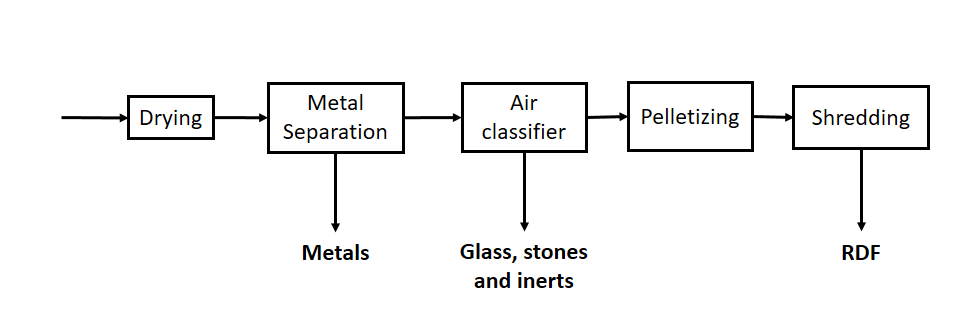
\includegraphics[width=0.5\columnwidth]{figs/fig9.png}
    \caption{}
    \label{fig9}
\end{figure}

\item With reference to the gate shown in \figref{fig10}, the gate will start opening automatically when the water level `h' above the hinge is \_\_\_\_\_\_\_ $m$ \textit{(rounded off to 2 decimal places)}.
\hfill\brak{GATE~ES~2025}
\begin{figure}[H]
    \centering
    
\includegraphics[width=0.5\columnwidth]{figs/fig10.png}
    \caption{}
    \label{fig10}
\end{figure}

\item In a cyclone separator of radius $25 cm$, a particle is travelling with a gas stream at velocity of $18 m/s$. The ratio of centrifugal force to the gravitational force acting on the particle is \_\_\_\_\_\_\_ \textit{(rounded off to 2 decimal places)}. Consider acceleration due to gravity ($g$) as $9.8 m/s^2$.
\hfill\brak{GATE~ES~2025}

\item Two sources of noise, adjacent to each other in a room, have sound pressure levels of 30 and 40 decibel (dB). The combined sound pressure level in the room is \_\_\_\_\_\_\_ dB \textit{(rounded off to 2 decimal places)}. Use reference sound pressure as 20 $\mu$Pa.
\hfill\brak{GATE~ES~2025}

\item An industrial stack emits $100 g/s$ of $CO$ at an effective height of `H', where the wind speed is $5 m/s$. At $3 km$ distance downwind, the values of dispersion coefficient in y direction and z-direction are $50 m$ and $25 m$, respectively. The $CO$ concentration at the centerline of the plume at $3 km$ distance downwind is \_\_\_\_\_\_\_ $mg/m^3$ \textit{(rounded off to 2 decimal places)}? Use Gaussian plume model and value of $\pi$ = 3.14. Neglect reactions and the ground effect of plume in the calculations.
\hfill\brak{GATE~ES~2025}

\item Two hypothetical organic waste streams $A$ and $B$ are mixed prior to the composting process. Waste-$A$ has 2.16\% of $C$ and 1.20\% of $N$. Waste-$B$ has 19.10\% of $C$ and 0.14\% of $N$. The quantity of Waste-$B$ that should be mixed with per kg of Waste-$A$ to achieve the desired $C:N$ ratio of 25 is \_\_\_\_\_\_\_ $kg$ \textit{(rounded off to 2 decimal places)}. Assume both the waste streams are completely dry.
\hfill\brak{GATE~ES~2025}

\item Food waste, paper waste and plastic waste have typical densities of $280 kg/m^3$, $80 kg/m^3$, and $50 kg/m^3$, respectively. The mixed waste is composed of 70\% food waste, 20\% paper waste and 10\% plastic waste. The density of the mixed waste is \_\_\_\_\_\_\_ $kg/m^3$ \textit{(rounded off to 2 decimal places)}. Neglect compaction effect.
\hfill\brak{GATE~ES~2025}

\item For a biodegradable waste with a chemical formula $C_{50}H_{100}O_{40}N$, the maximum theoretical methane production per ton of waste is \_\_\_\_\_\_\_ $kg$ \textit{(rounded off to 2 decimal places)}. Assume 100\% anaerobic conversion. Atomic weights of C-12; H-1; O-16; N-14.
\hfill\brak{GATE~ES~2025}

\item A person consumes 2.5 liters of water per day. The water quality test indicated that the supplied water has a $Pb$ concentration of $0.6 mg/L$. If the weight of the person is $75 kg$, the exposure level for $Pb$ for this person from this drinking water source is \_\_\_\_\_\_\_ $mg/kg/day$ \textit{(rounded off to 2 decimal places)}.
\hfill\brak{GATE~ES~2025}

\item In a region, total annual consumption of gasoline is 30.6 million tons. The land required for growing sugarcane to produce enough bioethanol to replace the gasoline completely is \_\_\_\_\_\_\_ $km^2$ \textit{(an integer value)}.
Ethanol energy equivalent is 67\% of gasoline, gasoline density is $850 kg/m^3$, yield of bioethanol produced from sugarcane per hectare of land is $3750 L$, and $1 km^2$ = 100 hectares.
\hfill\brak{GATE~ES~2025}

\item Initially a bottle contained $400 g$ of ethanol. Half of ethanol was used by a student for preparing the stock solution in an environmental chemistry laboratory just before summer vacation of 90 days. After completing the procedure, the student left the bottle uncorked. If the unsealed bottle losses ethanol at a rate of $0.5 g/day$, the ethanol that will be left in the bottle at the end of the summer vacation is \_\_\_\_\_\_\_ $g$ \textit{(an integer value)}.
\hfill\brak{GATE~ES~2025}
\end{enumerate}
\bigskip

\begin{align}
\textbf{END OF THE QUESTION PAPER}
\end{align}

\end{document}